%\VignetteIndexEntry{TNBC.CMS: prediction of TNBC consensus molecular subtype}
%\VignetteDepends{e1071, quadprog}
%\VignetteImports{GSVA, limma, pheatmap, grDevices, RColorBrewer, pracma}
%\VignettePackage{TNBC.CMS}
%\VignetteEngine{knitr::knitr}

%%%http://yihui.name/knitr/options/

\documentclass{article}\usepackage[]{graphicx}\usepackage[]{color}
%% maxwidth is the original width if it is less than linewidth
%% otherwise use linewidth (to make sure the graphics do not exceed the margin)
\makeatletter
\def\maxwidth{ %
  \ifdim\Gin@nat@width>\linewidth
    \linewidth
  \else
    \Gin@nat@width
  \fi
}
\makeatother

\definecolor{fgcolor}{rgb}{0.345, 0.345, 0.345}
\newcommand{\hlnum}[1]{\textcolor[rgb]{0.686,0.059,0.569}{#1}}%
\newcommand{\hlstr}[1]{\textcolor[rgb]{0.192,0.494,0.8}{#1}}%
\newcommand{\hlcom}[1]{\textcolor[rgb]{0.678,0.584,0.686}{\textit{#1}}}%
\newcommand{\hlopt}[1]{\textcolor[rgb]{0,0,0}{#1}}%
\newcommand{\hlstd}[1]{\textcolor[rgb]{0.345,0.345,0.345}{#1}}%
\newcommand{\hlkwa}[1]{\textcolor[rgb]{0.161,0.373,0.58}{\textbf{#1}}}%
\newcommand{\hlkwb}[1]{\textcolor[rgb]{0.69,0.353,0.396}{#1}}%
\newcommand{\hlkwc}[1]{\textcolor[rgb]{0.333,0.667,0.333}{#1}}%
\newcommand{\hlkwd}[1]{\textcolor[rgb]{0.737,0.353,0.396}{\textbf{#1}}}%
\let\hlipl\hlkwb

\usepackage{framed}
\makeatletter
\newenvironment{kframe}{%
 \def\at@end@of@kframe{}%
 \ifinner\ifhmode%
  \def\at@end@of@kframe{\end{minipage}}%
  \begin{minipage}{\columnwidth}%
 \fi\fi%
 \def\FrameCommand##1{\hskip\@totalleftmargin \hskip-\fboxsep
 \colorbox{shadecolor}{##1}\hskip-\fboxsep
     % There is no \\@totalrightmargin, so:
     \hskip-\linewidth \hskip-\@totalleftmargin \hskip\columnwidth}%
 \MakeFramed {\advance\hsize-\width
   \@totalleftmargin\z@ \linewidth\hsize
   \@setminipage}}%
 {\par\unskip\endMakeFramed%
 \at@end@of@kframe}
\makeatother

\definecolor{shadecolor}{rgb}{.97, .97, .97}
\definecolor{messagecolor}{rgb}{0, 0, 0}
\definecolor{warningcolor}{rgb}{1, 0, 1}
\definecolor{errorcolor}{rgb}{1, 0, 0}
\newenvironment{knitrout}{}{} % an empty environment to be redefined in TeX

\usepackage{alltt}
\usepackage{graphicx}
\usepackage{microtype}
\usepackage[T1]{fontenc}
\usepackage[latin1]{inputenc}
\usepackage{lmodern}
\usepackage{geometry}
\usepackage{authblk}
\usepackage{float}
\geometry{verbose,tmargin=2.5cm,bmargin=2.5cm,lmargin=2.5cm,rmargin=2.5cm}
\usepackage[table]{xcolor}
\IfFileExists{upquote.sty}{\usepackage{upquote}}{}
\begin{document}




\title{\texttt{TNBC.CMS}: prediction of TNBC consensus molecular subtype}

\author[1]{Doyeong Yu}
\author[1]{Jihyun Kim}
\author[2]{In Hae Park}
\author[1]{Charny Park}

\affil[1]{Clinical Genomics Analysis Branch, Research Institute, National Cancer Center, Gyeonggi-do, Republic of Korea}
\affil[2]{Center for Breast Cancer, Hospital, National Cancer Center, Gyeonggi-do, Republic of Korea}

\maketitle
\tableofcontents
\pagebreak
%------------------------------------------------------------
\section{Introduction}
%------------------------------------------------------------
Triple-negative breast cancer (TNBC) is a tumor with negative expression of estrogen receptor (ER), progesterone receptor (PR), and HER2. It is known to be a heterogeneous disease with poor prognosis, which makes the identification of molecular subtypes difficult. While previous studies proposed a different number of molecular subtypes, a reproducible and clinically relevant subtyping method has not been established yet.\paragraph{}
We developed a gene-expression based subtyping scheme to classify TNBC into four consensus molecular subtypes (CMS): mesenchymal-like(MSL), immunomodulatory (IM), luminal AR (LAR), and stem-like (SL). We identified the optimal number of molecular subtypes by consensus clustering, and built a support vector machine (SVM) classifier. Internal and external validation of our subtyping scheme confirmed its robustness and reproducibility.\paragraph{}
The \texttt{TNBC.CMS} package implements the SVM classifier to predict the consensus molecular subtypes of a triple negative breast cancer based on its gene expression profile. It also provides the functions for the characterization of the subtypes. In this vignette, we will illustrate how to assign the consensus molecular subtypes to TNBC samples and investigate their biological and clinical features using this package.
%------------------------------------------------------------
\section{Package installation}
%------------------------------------------------------------
To install the \texttt{TNBC.CMS} package, enter the following commands:
\begin{knitrout}
\definecolor{shadecolor}{rgb}{0.969, 0.969, 0.969}\color{fgcolor}\begin{kframe}
\begin{alltt}
\hlkwd{source}\hlstd{(}\hlstr{"http://bioconductor.org/biocLite.R"}\hlstd{)}
\hlkwd{biocLite}\hlstd{(}\hlstr{"TNBC.CMS"}\hlstd{)}
\end{alltt}
\end{kframe}
\end{knitrout}

%------------------------------------------------------------
\section{Case study}
%------------------------------------------------------------
\subsection{Data}
In this case study, we use the data from the Molecular Taxonomy of Breast Cancer Internation Consortium (METABRIC) to predict TNBC consensus molecular subtypes and perform further analysis. The METABRIC datasets of gene expression and clinical features were obtained from SYNAPSE. We filtered out samples which seemed to be positive for ER, PR, and HER2 based on immunohistochemistry results and the distribution of gene expression.\paragraph{}
First, we load the package and the processed expression data. The dataset includes a total of 24,368 genes and 299 samples. Note that rows and columns correspond to genes and samples, and row names must be gene symbols.
\begin{knitrout}
\definecolor{shadecolor}{rgb}{0.969, 0.969, 0.969}\color{fgcolor}\begin{kframe}
\begin{alltt}
\hlkwd{library}\hlstd{(TNBC.CMS)}
\end{alltt}


{\ttfamily\noindent\itshape\color{messagecolor}{\#\# Loading required package: e1071}}

{\ttfamily\noindent\itshape\color{messagecolor}{\#\# Loading required package: quadprog}}\begin{alltt}
\hlkwd{load}\hlstd{(}\hlstr{"D:/TNBC/data/METABRIC_processed_expression.rda"}\hlstd{)}
\hlkwd{dim}\hlstd{(exprMETABRIC)}
\end{alltt}
\begin{verbatim}
## [1] 24368   299
\end{verbatim}
\begin{alltt}
\hlstd{exprMETABRIC[}\hlnum{1}\hlopt{:}\hlnum{5}\hlstd{,} \hlnum{1}\hlopt{:}\hlnum{5}\hlstd{]}
\end{alltt}
\begin{verbatim}
##          MB-0316 MB-0658 MB-0420 MB-0906 MB-0249
## RERE         8.9     8.3     8.5     9.5     8.5
## RNF165       5.8     6.7     5.9     5.8     6.6
## CD049690     5.6     5.4     5.3     5.3     5.3
## BC033982     5.3     5.1     5.1     5.2     5.5
## PHF7         5.9     5.7     5.4     5.8     5.6
\end{verbatim}
\end{kframe}
\end{knitrout}

\subsection{Subtype prediction}
The \texttt{predictCMS} function assigns consensus molecular subtypes to TNBC samples based on a gene expression matrix. Input matrix should neither be scaled nor log-transformed. Class probabilities can be retrieved by accessing the \texttt{probabilities} attribute.
\begin{knitrout}
\definecolor{shadecolor}{rgb}{0.969, 0.969, 0.969}\color{fgcolor}\begin{kframe}
\begin{alltt}
\hlstd{predictions} \hlkwb{<-} \hlkwd{predictCMS}\hlstd{(exprMETABRIC)}
\hlkwd{table}\hlstd{(predictions)}
\end{alltt}
\begin{verbatim}
## predictions
## MSL  IM LAR  SL 
##  37  35 100 127
\end{verbatim}
\begin{alltt}
\hlkwd{head}\hlstd{(}\hlkwd{attr}\hlstd{(predictions,} \hlstr{"probabilities"}\hlstd{))}
\end{alltt}
\begin{verbatim}
##             MSL       IM   LAR       SL
## MB-0316 0.01236 0.634936 0.051 0.302068
## MB-0658 0.19212 0.127167 0.126 0.554456
## MB-0420 0.16387 0.004807 0.301 0.530475
## MB-0906 0.09181 0.119434 0.788 0.000863
## MB-0249 0.00048 0.000571 0.999 0.000186
## MB-0660 0.00107 0.000067 0.999 0.000006
\end{verbatim}
\end{kframe}
\end{knitrout}

\subsection{Subtype characterization}
The \texttt{TNBC.CMS} package includes several functions for studying characteristics of the consensus molecular subtypes. In this section, we walk through the analysis of the METABRIC gene expression dataset using these functions.\paragraph{}
The \texttt{computeGES} function calculates signature scores for the following 7 gene expression signatures: EMT (epithelial-mesencymal transition), stromal, immune, microenvironment, stemness, hormone, and CIN (chromosomal instability). For more details about the gene expression signatures, please see the manual page for \texttt{computeGES} function.\paragraph{}
As shown in Figure 1, this function also draws boxplots of signature scores with p-values of comparison among the subtypes. Stromal, immune, hormone, and stemness scores are significantly higher in MSL, IM, LAR, and SL subgroups than in other subgroups, respectively.
\begin{knitrout}
\definecolor{shadecolor}{rgb}{0.969, 0.969, 0.969}\color{fgcolor}\begin{kframe}
\begin{alltt}
\hlstd{resultGES} \hlkwb{<-} \hlkwd{computeGES}\hlstd{(}\hlkwc{exp.mat} \hlstd{= exprMETABRIC,} \hlkwc{pred} \hlstd{= predictions,} \hlkwc{rnaseq} \hlstd{= F)}
\hlstd{resultGES[,}\hlnum{1}\hlopt{:}\hlnum{4}\hlstd{]}
\end{alltt}
\begin{verbatim}
##                  MB-0316 MB-0658 MB-0420 MB-0906
## EMT                 7.67    7.76    7.88     7.9
## Stromal          4666.43 5823.17 5791.69  6086.4
## Immune           7752.93 7500.08 6011.18  7952.0
## Microenvironment    0.89    0.86    0.62     1.1
## Stemness            0.71    0.55    0.43     0.4
## Hormone             6.72    6.78    6.60     7.4
## CIN                 8.46    8.58    8.31     7.5
\end{verbatim}
\end{kframe}\begin{figure}[H]
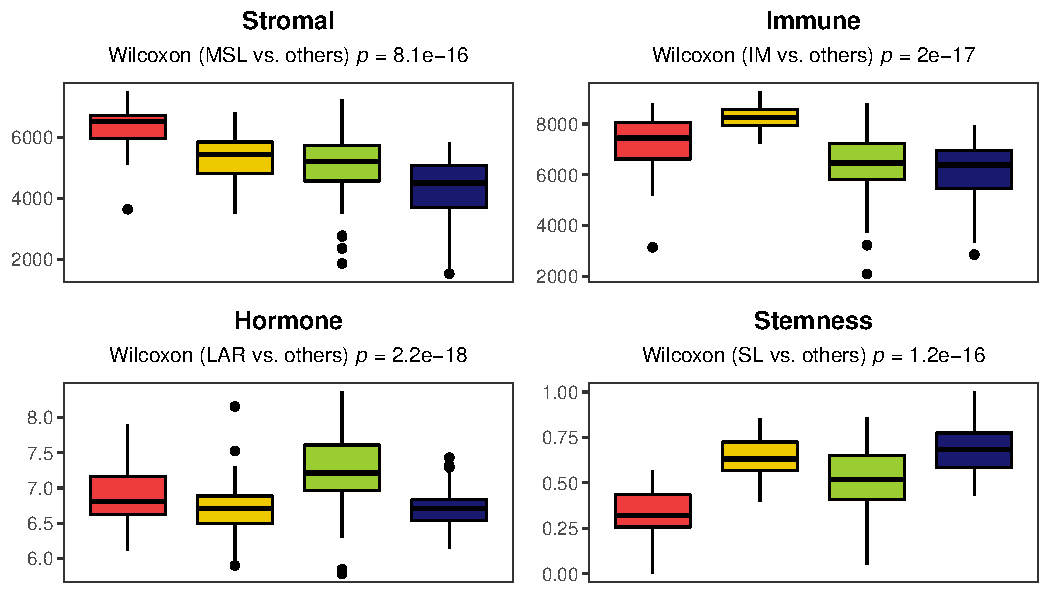
\includegraphics[width=\maxwidth]{figure/ges-1} \caption[Gene expression signature scores]{Gene expression signature scores}\label{fig:ges}
\end{figure}


\end{knitrout}

The \texttt{performGSVA} function performs gene set variation analysis on the hallmark gene sets and produces a heatmap representing GSVA enrichment scores. Figure 2 shows differential activation of the hallmark pathways across the subtypes. The MSL subtype has high levels of EMT and P53 pathway activation, and the IM subtype shows the highest inflammatory response. AR and ER response pathways are highly activated in the LAR subtpe, and the expression of cell cycle associated pathway genes is up-regulated in the SL subtype.
\begin{knitrout}
\definecolor{shadecolor}{rgb}{0.969, 0.969, 0.969}\color{fgcolor}\begin{kframe}
\begin{alltt}
\hlstd{resultGSVA} \hlkwb{<-} \hlkwd{performGSVA}\hlstd{(}\hlkwc{exp.mat} \hlstd{= exprMETABRIC,} \hlkwc{pred} \hlstd{= predictions)}
\hlkwd{head}\hlstd{(resultGSVA[,}\hlnum{1}\hlopt{:}\hlnum{4}\hlstd{])}
\end{alltt}
\begin{verbatim}
##                                   MB-0316 MB-0658 MB-0420 MB-0906
## KRAS_SIGNALING                      0.013   0.095    0.15   0.138
## COAGULATION                         0.214   0.137    0.28   0.288
## EPITHELIAL_MESENCHYMAL_TRANSITION  -0.299   0.238    0.50   0.270
## MYOGENESIS                         -0.196   0.029    0.18   0.186
## ANGIOGENESIS                       -0.269   0.199    0.43  -0.100
## APICAL_JUNCTION                    -0.138   0.096    0.28   0.022
\end{verbatim}
\end{kframe}\begin{figure}[H]
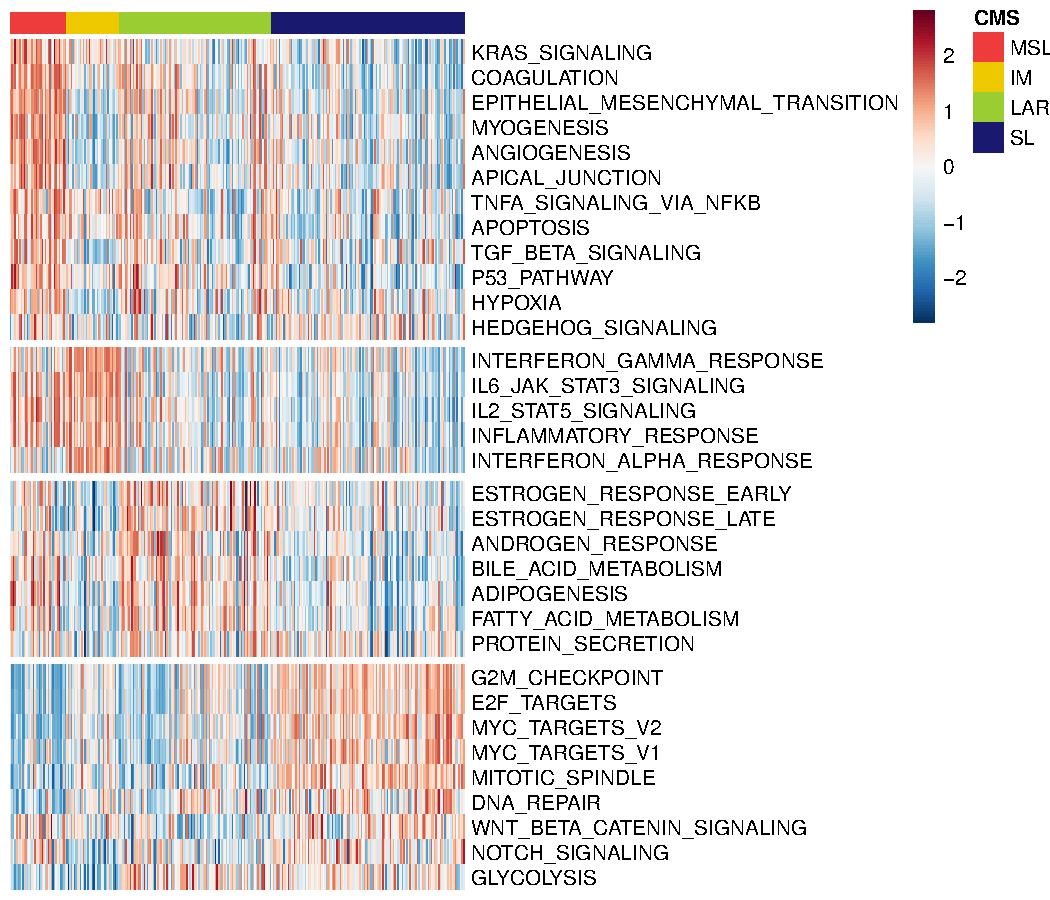
\includegraphics[width=\maxwidth]{figure/gsa-1} \caption[GSVA enrichment scores]{GSVA enrichment scores}\label{fig:gsa}
\end{figure}


\end{knitrout}

The \texttt{TNBC.CMS} package provides two functions for survival analysis: \texttt{plotKM} and \texttt{plotHR}. Here, we use the five-year survival data from the METABRIC dataset to study the association between overall survival and the consensus molecular subtypes.\paragraph{}
The \texttt{plotKM} function produces a Kaplan-Meier curve for each consensus molecular subtype like Figure 3. The MSL subtype had significantly better prognosis than other subtypes while the SL group showed the worst prognosis, which is consistent with our previous study.
\begin{knitrout}
\definecolor{shadecolor}{rgb}{0.969, 0.969, 0.969}\color{fgcolor}\begin{kframe}
\begin{alltt}
\hlkwd{load}\hlstd{(}\hlstr{"D:/TNBC/data/METABRIC_clinical_features.rda"}\hlstd{)}
\hlkwd{plotKM}\hlstd{(}\hlkwc{pred} \hlstd{= predictions,} \hlkwc{time} \hlstd{= clinMETABRIC}\hlopt{$}\hlstd{OS5_MONTHS,} \hlkwc{event} \hlstd{= clinMETABRIC}\hlopt{$}\hlstd{OS5_STATUS)}
\end{alltt}
\end{kframe}\begin{figure}[H]

{\centering 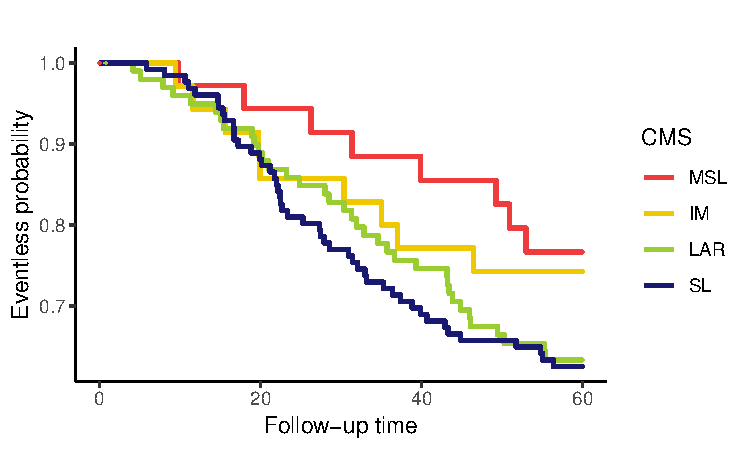
\includegraphics[width=\maxwidth]{figure/os-1} 

}

\caption[Overall survival]{Overall survival}\label{fig:os}
\end{figure}


\end{knitrout}

The \texttt{plotHR} produces a forest plot of hazard ratios for genes that the user provides. For each input gene, samples are divided into high and low groups based on its expression and the 95\% confidence interval for the hazard ratio is calculated.
\begin{knitrout}
\definecolor{shadecolor}{rgb}{0.969, 0.969, 0.969}\color{fgcolor}\begin{kframe}
\begin{alltt}
\hlstd{gs1} \hlkwb{<-} \hlkwd{c}\hlstd{(}\hlstr{"ENC1"}\hlstd{,} \hlstr{"PLK2"}\hlstd{,} \hlstr{"BQ015566"}\hlstd{,} \hlstr{"PDZD8"}\hlstd{,} \hlstr{"TMEM176A"}\hlstd{,} \hlstr{"DEF6"}\hlstd{,} \hlstr{"SPATA17"}\hlstd{,} \hlstr{"CCND2"}\hlstd{)}
\hlkwd{plotHR}\hlstd{(}\hlkwc{exp.mat} \hlstd{= exprMETABRIC,} \hlkwc{gene.symbol} \hlstd{= gs1,} \hlkwc{pred} \hlstd{= predictions,}
       \hlkwc{time} \hlstd{= clinMETABRIC}\hlopt{$}\hlstd{OS5_MONTHS,} \hlkwc{event} \hlstd{= clinMETABRIC}\hlopt{$}\hlstd{OS5_STATUS,} \hlkwc{by.subtype} \hlstd{= F)}
\end{alltt}
\end{kframe}\begin{figure}[H]
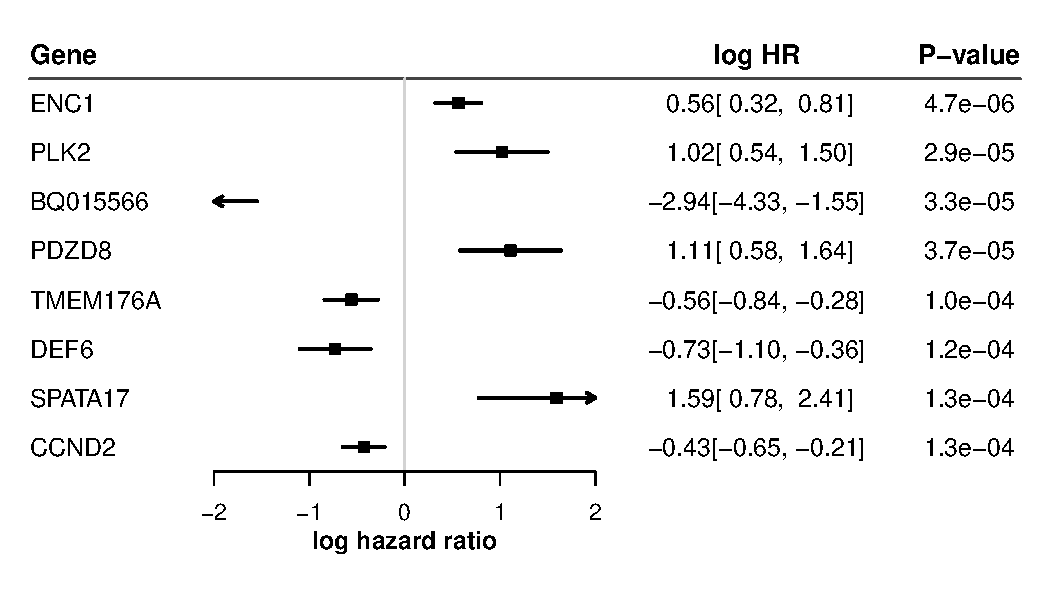
\includegraphics[width=\maxwidth]{figure/hr-1} \caption[Forest plot of hazard ratios]{Forest plot of hazard ratios}\label{fig:hr}
\end{figure}


\end{knitrout}

Also, subtype-specific hazard ratios for genes of interest can be computed by setting the \texttt{by.subtype} argument.
\begin{knitrout}
\definecolor{shadecolor}{rgb}{0.969, 0.969, 0.969}\color{fgcolor}\begin{kframe}
\begin{alltt}
\hlstd{gs2} \hlkwb{<-} \hlkwd{c}\hlstd{(}\hlstr{"AKAP12"}\hlstd{,} \hlstr{"BTK"}\hlstd{,} \hlstr{"CCR7"}\hlstd{,} \hlstr{"CD19"}\hlstd{)}
\hlkwd{plotHR}\hlstd{(}\hlkwc{exp.mat} \hlstd{= exprMETABRIC,} \hlkwc{gene.symbol} \hlstd{= gs2,} \hlkwc{pred} \hlstd{= predictions,}
       \hlkwc{time} \hlstd{= clinMETABRIC}\hlopt{$}\hlstd{OS5_MONTHS,} \hlkwc{event} \hlstd{= clinMETABRIC}\hlopt{$}\hlstd{OS5_STATUS,} \hlkwc{by.subtype} \hlstd{= T)}
\end{alltt}
\end{kframe}\begin{figure}[H]
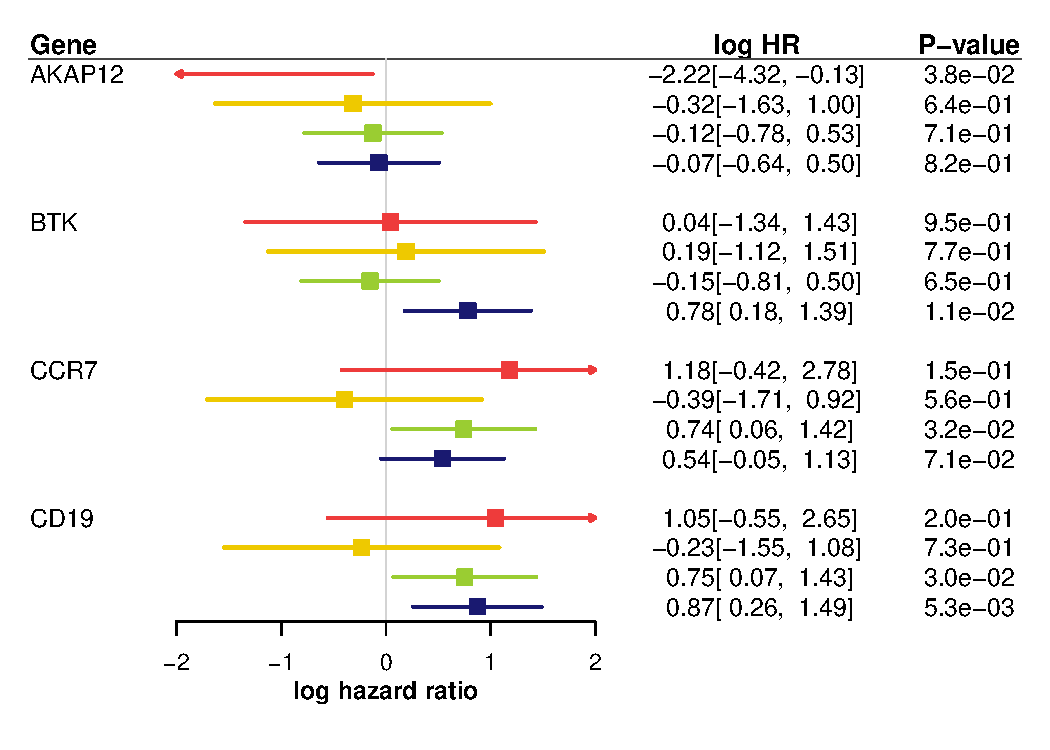
\includegraphics[width=\maxwidth]{figure/hrsub-1} \caption[Forest plot of subtype-specific hazard ratios]{Forest plot of subtype-specific hazard ratios}\label{fig:hrsub}
\end{figure}


\end{knitrout}

The \texttt{computeDS} function computes drug signature scores for the corresponding gene sets in the MSigDB CGP (chemical and genetic perturbations) collection and draws a heatmap of the signature scores (Figure 3). The MSL and SL subtypes appear to be resistant to cisplatin and doxorubicin, respectively. Also, the IM and LAR subtypes show higher levels of signature scores for androgen agonist and SB216763 (an inhibitor of GSK3B) than other subtypes, respectively.
\begin{knitrout}
\definecolor{shadecolor}{rgb}{0.969, 0.969, 0.969}\color{fgcolor}\begin{kframe}
\begin{alltt}
\hlstd{resultDS} \hlkwb{<-} \hlkwd{computeDS}\hlstd{(}\hlkwc{exp.mat} \hlstd{= exprMETABRIC,} \hlkwc{pred} \hlstd{= predictions)}
\hlkwd{head}\hlstd{(resultDS[,}\hlnum{1}\hlopt{:}\hlnum{4}\hlstd{])}
\end{alltt}
\begin{verbatim}
##              MB-0316 MB-0658 MB-0420 MB-0906
## APLIDIN        -0.32   -0.27   -0.26    0.15
## CISPLATIN      -0.57   -0.51   -0.99   -0.86
## DASATINIB      -0.99   -0.84   -1.06   -0.61
## FORSKOLIN       7.81    7.88    7.81    7.82
## IMATINIB       -7.47   -7.43   -7.81   -7.56
## TROGLITAZONE    7.65    7.94    7.40    8.21
\end{verbatim}
\end{kframe}\begin{figure}[H]
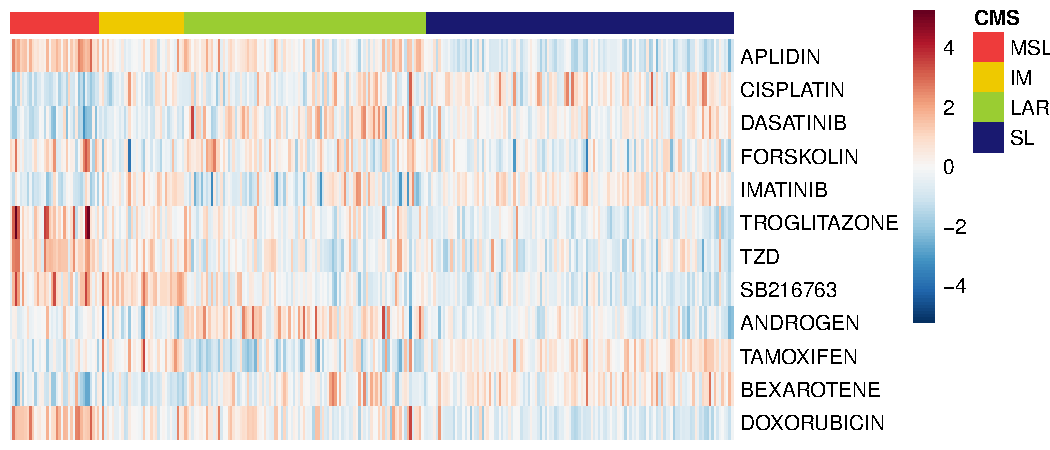
\includegraphics[width=\maxwidth]{figure/ds-1} \caption[Drug signature scores]{Drug signature scores}\label{fig:ds}
\end{figure}


\end{knitrout}

%------------------------------------------------------------
\section{Session Info}
%------------------------------------------------------------
\begin{knitrout}
\definecolor{shadecolor}{rgb}{0.969, 0.969, 0.969}\color{fgcolor}\begin{kframe}
\begin{alltt}
\hlkwd{sessionInfo}\hlstd{()}
\end{alltt}
\begin{verbatim}
## R version 3.4.4 (2018-03-15)
## Platform: x86_64-w64-mingw32/x64 (64-bit)
## Running under: Windows 7 x64 (build 7601) Service Pack 1
## 
## Matrix products: default
## 
## locale:
## [1] LC_COLLATE=Korean_Korea.949  LC_CTYPE=Korean_Korea.949   
## [3] LC_MONETARY=Korean_Korea.949 LC_NUMERIC=C                
## [5] LC_TIME=Korean_Korea.949    
## 
## attached base packages:
## [1] stats     graphics  grDevices utils     datasets  methods   base     
## 
## other attached packages:
## [1] TNBC.CMS_0.1.0 quadprog_1.5-5 e1071_1.7-0.1  knitr_1.21    
## 
## loaded via a namespace (and not attached):
##  [1] Biobase_2.38.0       bit64_0.9-7          splines_3.4.4       
##  [4] R.utils_2.7.0        shiny_1.2.0          assertthat_0.2.0    
##  [7] highr_0.7            stats4_3.4.4         blob_1.1.1          
## [10] lattice_0.20-35      pillar_1.3.1         RSQLite_2.1.1       
## [13] backports_1.1.3      glue_1.3.0           digest_0.6.18       
## [16] RColorBrewer_1.1-2   promises_1.0.1       checkmate_1.9.1     
## [19] colorspace_1.4-0     Matrix_1.2-12        htmltools_0.3.6     
## [22] httpuv_1.4.5.1       R.oo_1.22.0          plyr_1.8.4          
## [25] GSEABase_1.40.1      XML_3.98-1.16        pkgconfig_2.0.2     
## [28] pheatmap_1.0.12      purrr_0.2.5          xtable_1.8-3        
## [31] scales_1.0.0         later_0.7.5          pracma_2.2.2        
## [34] tibble_2.0.1         GSVA_1.26.0          annotate_1.56.2     
## [37] IRanges_2.12.0       ggplot2_3.1.0        ggpubr_0.2          
## [40] BiocGenerics_0.24.0  lazyeval_0.2.1       survival_2.43-3     
## [43] magrittr_1.5         crayon_1.3.4         mime_0.6            
## [46] memoise_1.1.0        evaluate_0.12        GGally_1.4.0        
## [49] R.methodsS3_1.7.1    class_7.3-14         graph_1.56.0        
## [52] tools_3.4.4          stringr_1.3.1        S4Vectors_0.16.0    
## [55] munsell_0.5.0        AnnotationDbi_1.40.0 bindrcpp_0.2.2      
## [58] compiler_3.4.4       rlang_0.3.1          grid_3.4.4          
## [61] RCurl_1.95-4.11      rstudioapi_0.9.0     labeling_0.3        
## [64] bitops_1.0-6         gtable_0.2.0         DBI_1.0.0           
## [67] reshape_0.8.8        forestplot_1.7.2     R6_2.3.0            
## [70] dplyr_0.7.8          bit_1.1-14           bindr_0.1.1         
## [73] shinythemes_1.1.2    stringi_1.2.4        parallel_3.4.4      
## [76] Rcpp_1.0.0           geneplotter_1.56.0   tidyselect_0.2.5    
## [79] xfun_0.4
\end{verbatim}
\end{kframe}
\end{knitrout}

%------------------------------------------------------------
\section{References}
%------------------------------------------------------------
\begin{description}
\item Aran,D. et al. (2017) xCell: digitally portraying the tissue cellular heterogeneity landscape. \emph{Genome biology},18,220.
\item Carter,S.L. et al. (2006) A signature of chromosomal instability inferred from gene expression profiles predicts clinical outcome in multiple human cancers. \textit{Nature genetics},38,1043.
\item Malta,T.M. et al. (2018) Machine learning identifies stemness features associated with oncogenic dedifferentiation. \textit{Cell},173,338-354.
\item Tan,T.Z. et al. (2014) Epithelial-mesenchymal transition spectrum quantification and its efficacy in deciphering survival and drug responses of cancer patients. \textit{EMBO molecular medicine},6,1279-93.
\item Yoshihara,K. et al. (2013) Inferring tumour purity and stromal and immune cell admixture from expression data. \textit{Nature communications},4,2612.

\end{description}

\end{document}
